\documentclass[]{article}
\usepackage{graphicx}
\usepackage{amsmath,amsfonts,amssymb}
\usepackage[many]{tcolorbox}
\usepackage[%
margin=2cm,
includefoot,
bottom=2.55cm,
top=2.025cm,
headsep=0.5cm,
footskip=0.65cm
]{geometry}

\definecolor{myblue}{RGB}{0,46,142}

\newtcolorbox[auto counter]{mytheorem}[1][]{%
	enhanced jigsaw,
	colback=white,
	colframe=myblue,
	coltitle=myblue,
	fonttitle=\bfseries,
	sharp corners,
	detach title,
	enlarge left by=18mm,
	width=\linewidth-18mm,
	underlay unbroken and first={%
		\node[above,text=myblue,font=\bfseries,align=center] at ([xshift=-.5\textwidth,yshift=-7mm]interior.north) {\thetcbcounter};
	},
	breakable,
	pad at break=1mm,
	#1,
	code={\ifdefempty{\tcbtitletext}{}{\tcbset{before upper={\tcbtitle\par\medskip}}}},
}
\graphicspath{ {./images/} }


%opening
\title{L-17: Orthogonal Matrices and Gram Schmidt}
\author{Aahan Singh Charak\\Computer Science Grad}

\begin{document}
	\maketitle
	\section{Orthogonal Matrices}
	\vspace{10pt}
	
	\subsection{Orthonormal Vectors}
	\vspace{10pt}
	Unit vectors which are prependicular to each other are called orthonormal vectors.\\
	
	\noindent
	\[ 
	{q_i}^T.q_j=
	\begin{cases} 
		0 & if \ i\neq j \\
		1 & if \ i=j \\ 
	\end{cases}
	\]\\
	
	\noindent
	The self dot product is 1 as it is a unit vector. So length squared is zero.\\
	
	\vspace{10pt}
	\subsection{What are orthogonal matrices?}
	\vspace{10pt}
	
	Consider an n-dimensional vector space with n orthogonal basis $q_1,q_2,q_3...q_n$\\
	
	\noindent
	The orthogonal matrices has these basis vectors in its columns.\\
	
	\noindent
	$Q=[q_1  \ q_2 \ .... \ q_n]$\\
	
	\noindent
	\[
	Q_T.Q=\begin{bmatrix}
		{q_1}^T\\
		.\\
		.\\
		{q_n}^T
	\end{bmatrix}[q_1  \ q_2 \ .... \ q_n]=I
	\]\\
	
	\noindent
	Solve the identity proof yourself.
	
\vspace{10pt}

\subsection{Examples of orthogonal matrices}
\vspace{10pt}
\begin{itemize}
	\item[1)] \[
	Q=\begin{bmatrix}
		0&0&1\\
		1&0&0\\
		0&1&0
	\end{bmatrix}
	\]
	\item[2)]\[
	Q=\begin{bmatrix}
		\cos{\theta} & -\sin{\theta}\\
		\sin{\theta} & \cos{\theta}
	\end{bmatrix}
	\]
	\item[3)]\[
	Q=\frac{1}{2}\begin{bmatrix}
		1&1&1&1\\
		1&-1&1&-1\\
		1&1&-1&-1\\
		1&-1&-1&1
	\end{bmatrix}
	\]
	\item[4)]Rectangular example.\[
	 Q=\frac{1}{3}\begin{bmatrix}
	 	1&-2\\
	 	2&-1\\
	 	2&2
	 \end{bmatrix}
	\]
\end{itemize}

\vspace{10pt}

\subsection{Some properties}
\vspace{10pt}

Suppose Q is an orthogonal matrix with orthonormal vectors as its columns. Projection matrix for projecting a vector b onto its column space is given by:\\

\noindent
$P=Q{(Q^TQ)}^{-1}Q^T$\\

\noindent
$P=QQ^T$\\

\noindent
Now, suppose Q is an orthogonal matrix. All columns are orthonormal and independent. This means in an n dimensional space, we get n pivots after elimination. So the column space will be the entire n dimensional space.\\

\noindent
In this case P=I, as we won't have the need to project a vector as it would be already in the n-dimensional space. We can verify properties like $P^T=P \ and \ P^2=P$.\\

\vspace{10pt}

\subsection{Normal Equation}

\vspace{10pt}

$A^TA\hat{x}=A^Tb$\\
$Q^TQ\hat{x}=Q^Tb$\\

\noindent
$\hat{x}=Q^Tb$\\

\noindent
$\hat{x_i}={q_i}^Tb$ [i=ith component]\\

%Gram schmidt matrices
\vspace{10pt}
\section{Gram Schmidt Process}
In mathematics, particularly linear algebra and numerical analysis, the Gram–Schmidt process is a method for orthonormalizing a set of vectors in an inner product space, most commonly the Euclidean space $R^n$ equipped with the standard inner product.

\vspace{10pt}

\subsection{Two dimensional intuition}
\vspace{10pt}

\vspace{12pt}
\begin{center}
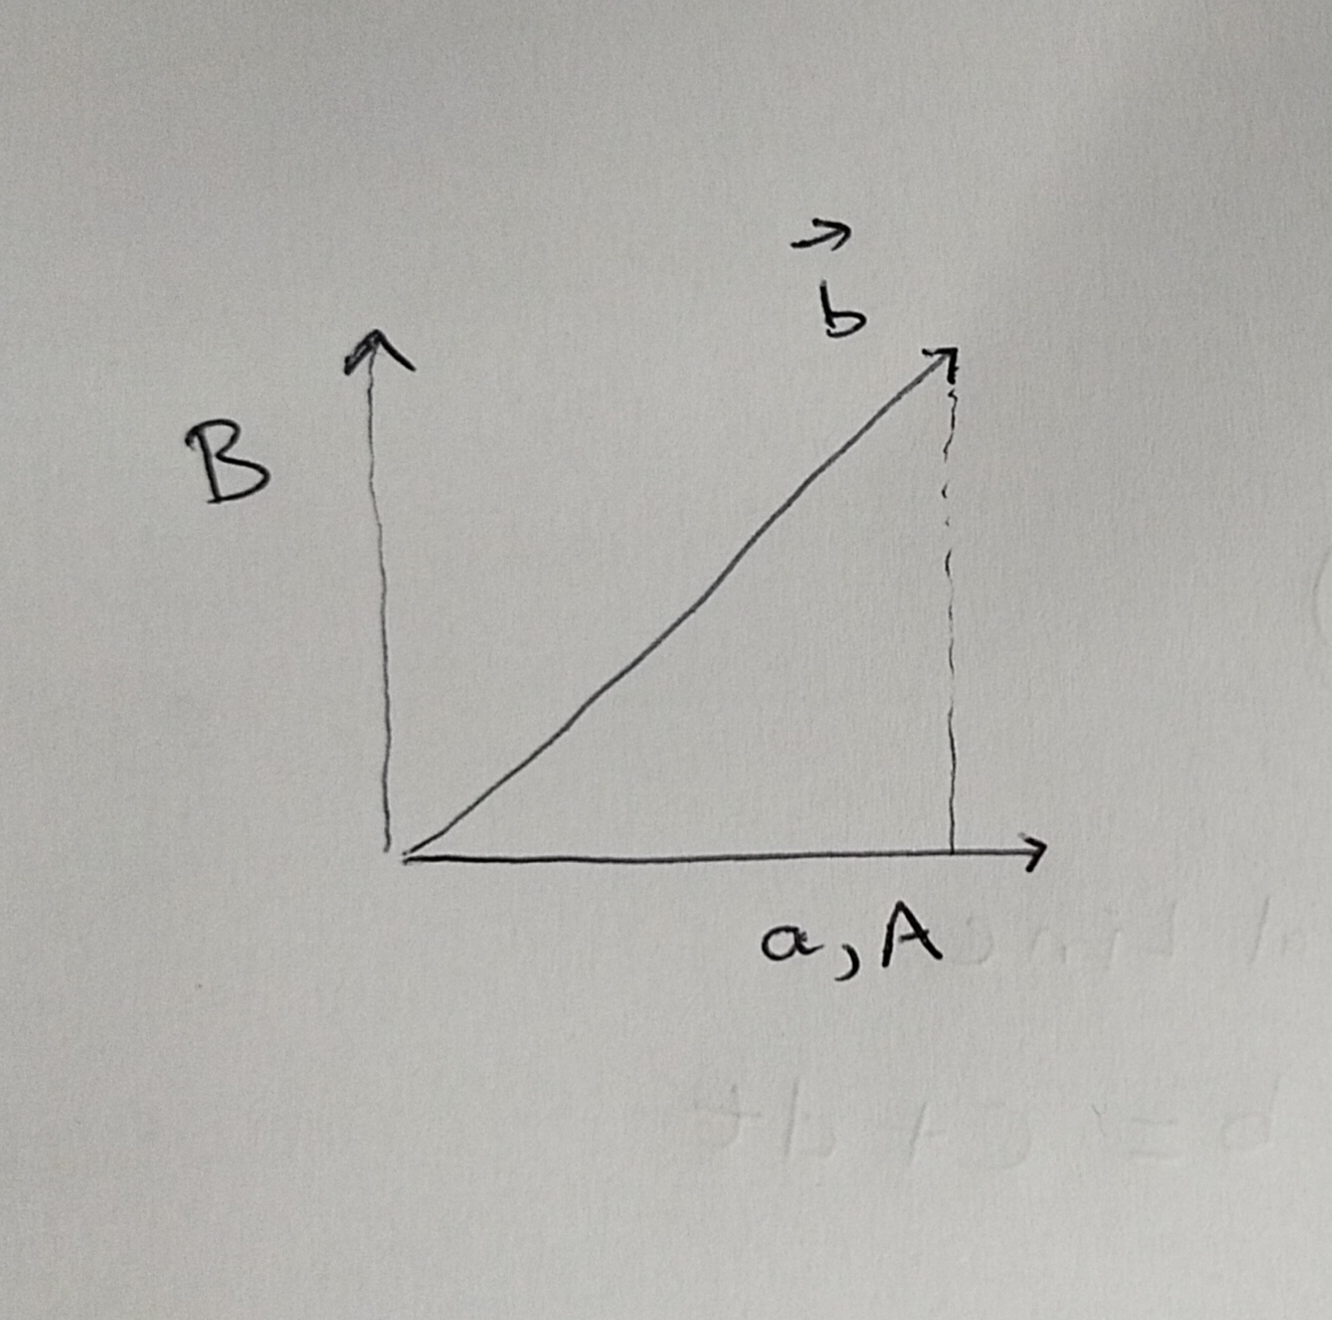
\includegraphics[scale=.25]{gram1}
\end{center}
\vspace{10pt}

\noindent
We have to make both vectors orthogonal. Lets take a vector as reference. Let's say say vector A is equal to a.\\


\noindent
Suppose B is perpendicular to A vector.\\

\noindent
B is the error projection of b.\\
Therefore, B=e\\

\noindent
B=b-e [parallelogram law]\\

\noindent
B=$b-\hat{x}a$[Proved in projection onto subspace lecture]\\
Or\\
$B=b-\hat{x}A$\\

\noindent
$\therefore B=b-\frac{A^Tb}{A^TA}A$ [Gram's formula] \\

\vspace{10pt}

\subsection{Three dimensional intuition}
\vspace{10pt}

\vspace{12pt}
\begin{center}
	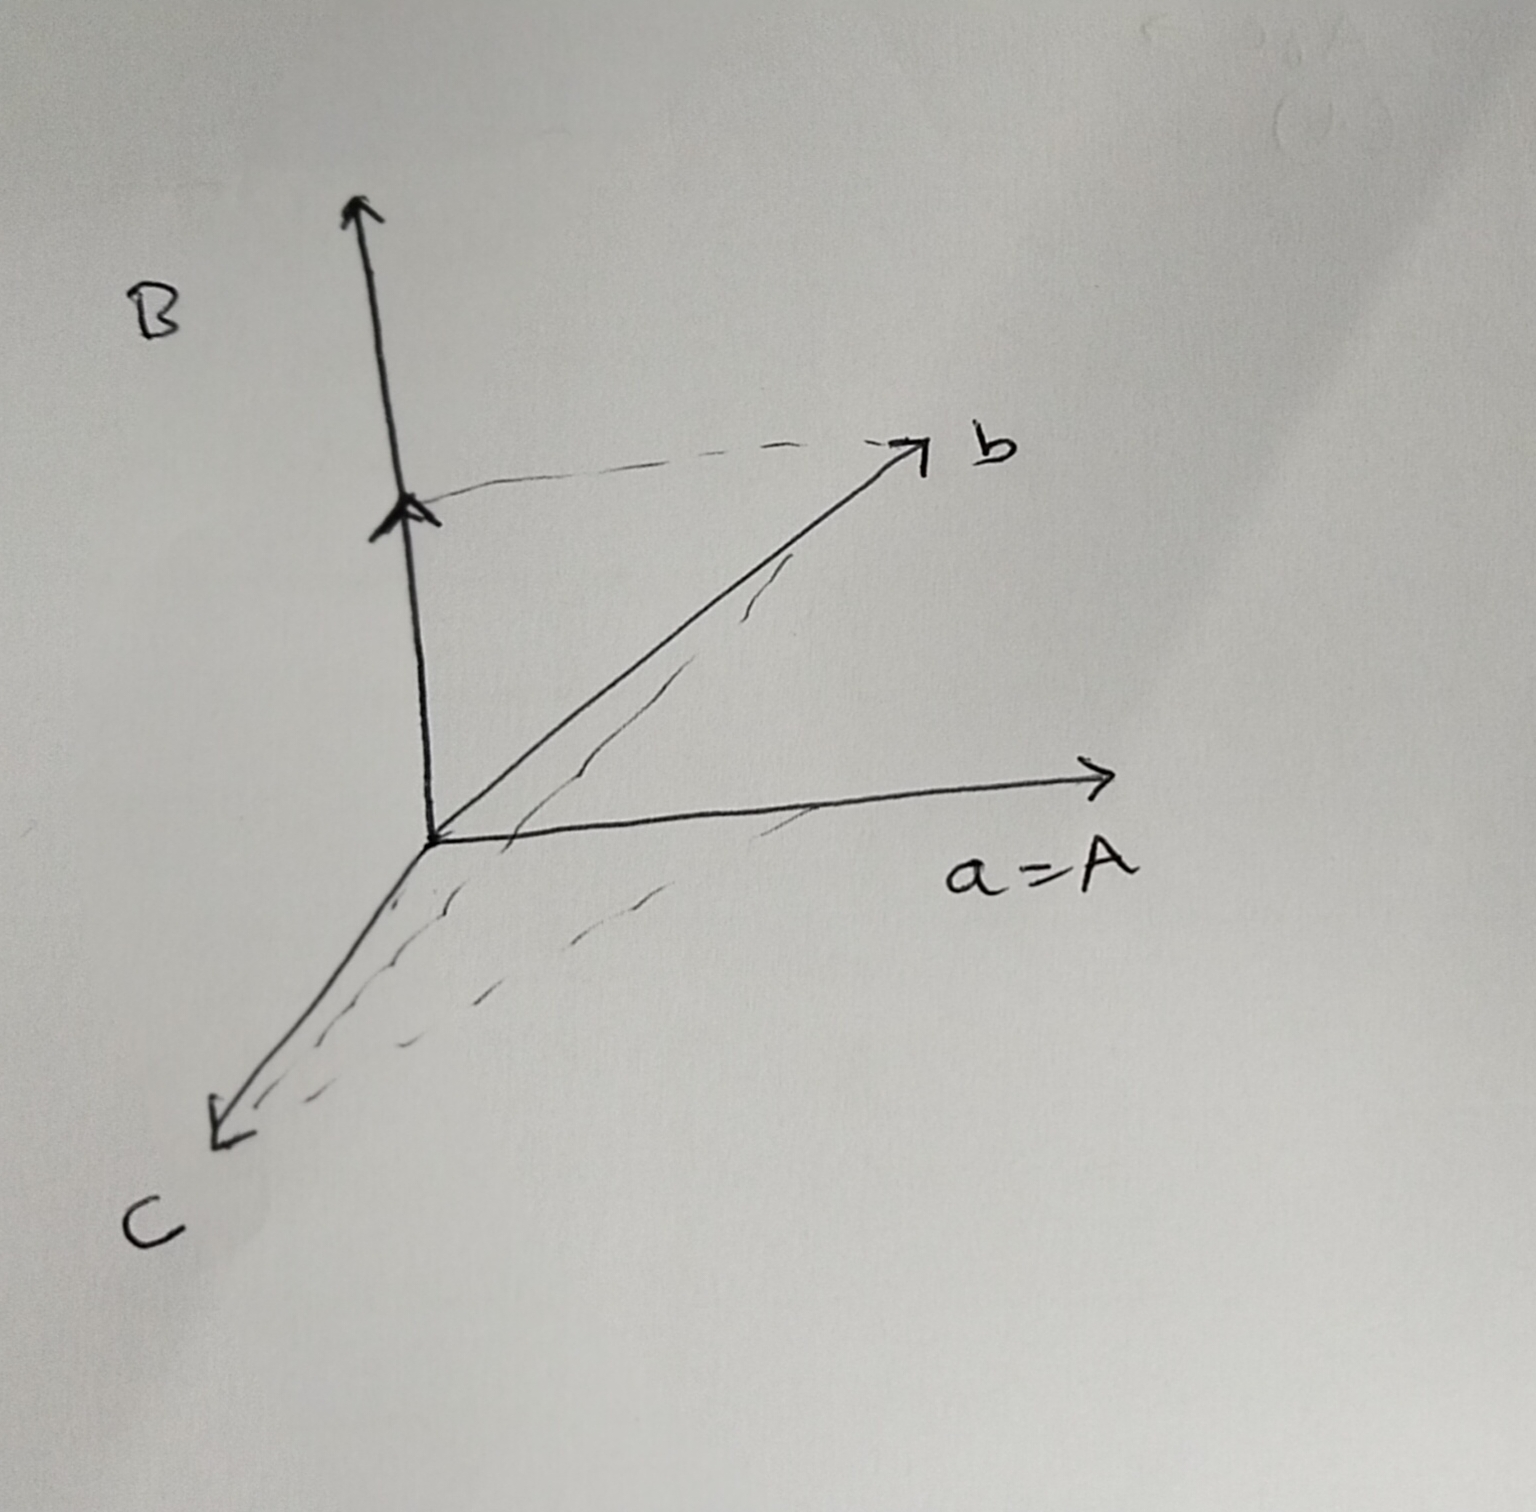
\includegraphics[scale=.25]{gram2}
\end{center}
\vspace{10pt}
\noindent
Here, $A \perp B \perp C$\\

\noindent
Like 2d intuition, A=a and $B=b-\frac{A^Tb}{A^TA}A$\\

\noindent
For C, we have to think differently.\\

\noindent
Projection of C on A is given by,
$p_1=\frac{A^Tc}{A^TA}A$\\

\noindent
Projection of C on B is given by,
$p_2=\frac{B^Tc}{B^TB}B$

\noindent
Now, these two vectors are perpendicular as A and B are perpendicular. They will become basis for a plane. A vector line on the plane would be linear combination of the above mentioned vectors, which is:\\

\noindent
$p_plane=p1+p2$\\

\noindent
Now, this is equivalent to projection of c on that plane. The perpendicular vector is given by:\\

\noindent
$C=c-(\frac{A^Tc}{A^TA}A) - (\frac{B^Tc}{B^TB}B)$\\

\vspace{10pt}

\section{Extra}
\vspace{10pt}
\subsection{Numerical Example}
\vspace{10pt}
\[
a=\begin{bmatrix}
	1\\
	1\\
	1\\
\end{bmatrix}, b=\begin{bmatrix}
1\\
0\\
2
\end{bmatrix}, S=\begin{bmatrix}
1&1\\
1&0\\
1&2
\end{bmatrix}
\]\\

\noindent
\[
B=\begin{bmatrix}
	1\\
	0\\
	2
\end{bmatrix}-\frac{3}{3}\begin{bmatrix}
1\\
1\\
1
\end{bmatrix}
\]\\

\noindent
\[
B=\begin{bmatrix}
	0\\
	-1\\
	1
\end{bmatrix}
\]\\

\noindent
\[
Q=[q1,q2]
\]\\

\noindent
\[
Q=\begin{bmatrix}
	\frac{1}{\sqrt{3}}&0\\
	\frac{1}{\sqrt{3}}&\frac{-1}{\sqrt{2}}\\
	\frac{1}{\sqrt{3}}&\frac{1}{\sqrt{2}}
\end{bmatrix}
\]
\vspace{10pt}

\subsection{Relation between C(Q) and C(S)}
\vspace{10pt}	
The column space of both matrices is the same. A and B are perpendicular. They form a 2d column space. It's just that Q matrix is more refined than the above mentioned vectors,as it contains unit vectors in the directions of A and B. Thus, it has basis for C(S).


\end{document}